%
% dq.tex
%
% (c) 2021 Prof Dr Andreas Müller, OST Ostschweizer Fachhochschule
%
\documentclass[tikz]{standalone}
\usepackage{times}
\usepackage{amsmath}
\usepackage{txfonts}
\usepackage[utf8]{inputenc}
\usepackage{graphics}
\usetikzlibrary{arrows,intersections,math}
\usepackage{ifthen}
\begin{document}

\definecolor{darkred}{rgb}{0.7,0,0}

\newboolean{showgrid}
\setboolean{showgrid}{false}
\def\breite{6}
\def\hoehe{6}

\begin{tikzpicture}[>=latex,thick]

% Povray Bild
\node at (0,0) {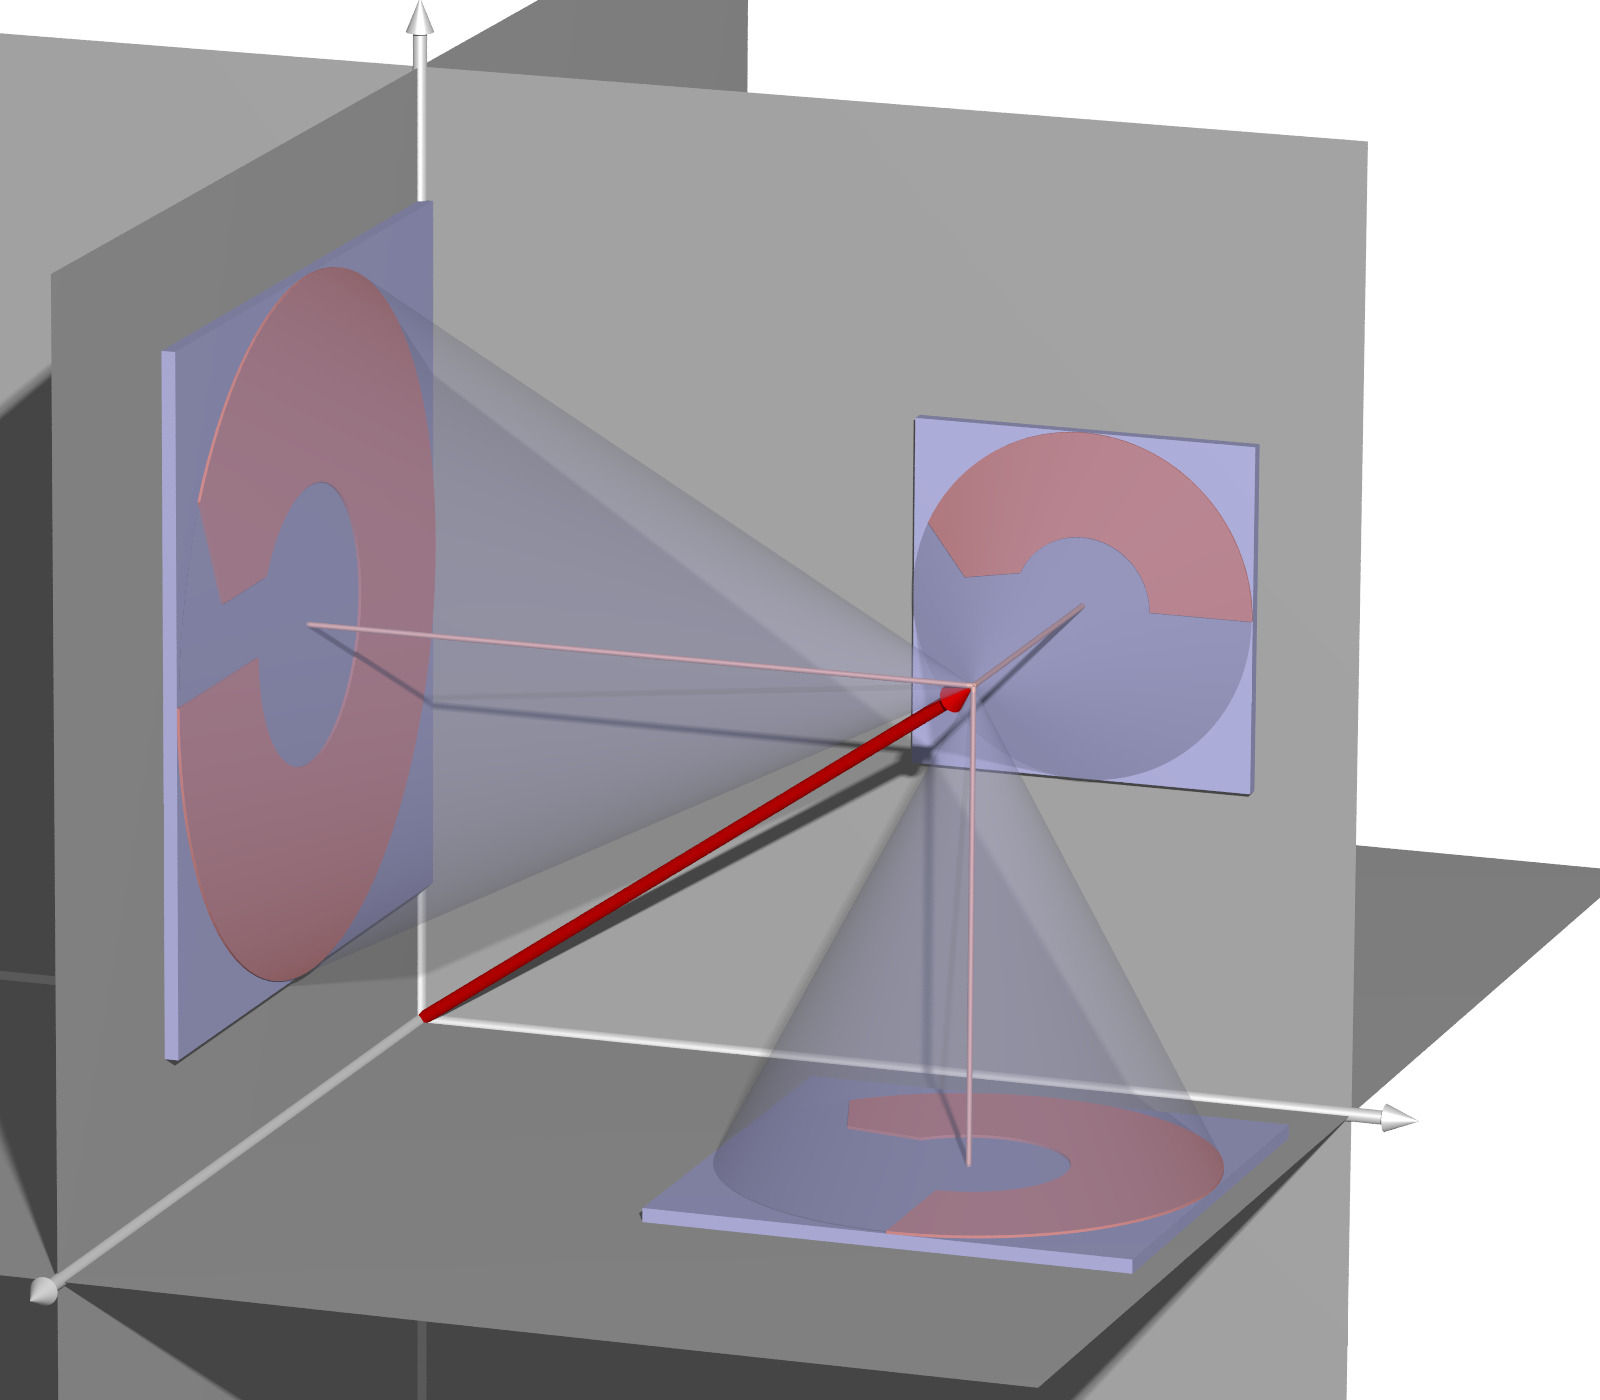
\includegraphics[width=12cm]{dq.jpg}};

% Gitter
\ifthenelse{\boolean{showgrid}}{
\draw[step=0.1,line width=0.1pt] (-\breite,-\hoehe) grid (\breite, \hoehe);
\draw[step=0.5,line width=0.4pt] (-\breite,-\hoehe) grid (\breite, \hoehe);
\draw                            (-\breite,-\hoehe) grid (\breite, \hoehe);
\fill (0,0) circle[radius=0.05];
}{}

\node at (-2.8,-2.7) {$O$};
\node at (4.7,-3.4) {$a_1$};
\node at (-2.6,5.2) {$a_2$};
\fill[color=white,opacity=0.7] ({-5.7-0.25},{-4.8-0.15}) rectangle ({-5.7+0.25},{-4.8+0.2});
\node at (-5.7,-4.8) {$a_3$};

\node[color=blue] at (-3.6,0.8) {$y\mathbf{e}_{23}$};
\node[color=blue] at (2.1,0.9) {$x\mathbf{e}_{12}$};
\node[color=blue] at (1.3,-3.7) {$z\mathbf{e}_{13}$};

\node[color=darkred] at (1.3,0.4) {$\vec{q}$};

\end{tikzpicture}

\end{document}

